\documentclass[10.5pt,a4paper]{article}
\usepackage[margin=1.8cm]{geometry}
\usepackage{fontspec}
\setmainfont{DejaVu Sans}
\setmonofont{DejaVu Sans Mono}[Scale=0.9]
\usepackage{unicode-math}
\setmathfont{DejaVu Math TeX Gyre}
\usepackage{graphicx,enumitem,xcolor}
\pagestyle{empty}
\setlength{\parindent}{0pt}
\setlist[enumerate]{label=\alph*),leftmargin=1.4em,itemsep=0pt}
\newcommand{\resp}[1]{\par\vspace{#1}}
\newcommand{\preg}[1]{\vspace{4pt}{\large\bfseries #1}\par\vspace{3pt}}
\begin{document}
{\Large\bfseries SI7011 · Evento evaluativo 1 · Parte A: leer la evidencia}\par\vspace{10pt}
\textbf{Nombre:} \rule{8cm}{0.4pt}\hfill\textbf{Documento:} \rule{4cm}{0.4pt}\par\vspace{8pt}
\textbf{Individual · sin computador ni apuntes · 30 minutos · 6 preguntas, 1 punto cada una.}
Respuestas cortas: una o dos frases por literal. Cuando la pregunta pide evidencia, cita un número leído de la figura.
\vspace{6pt}\hrule\vspace{6pt}

\preg{1. Dos corridas}
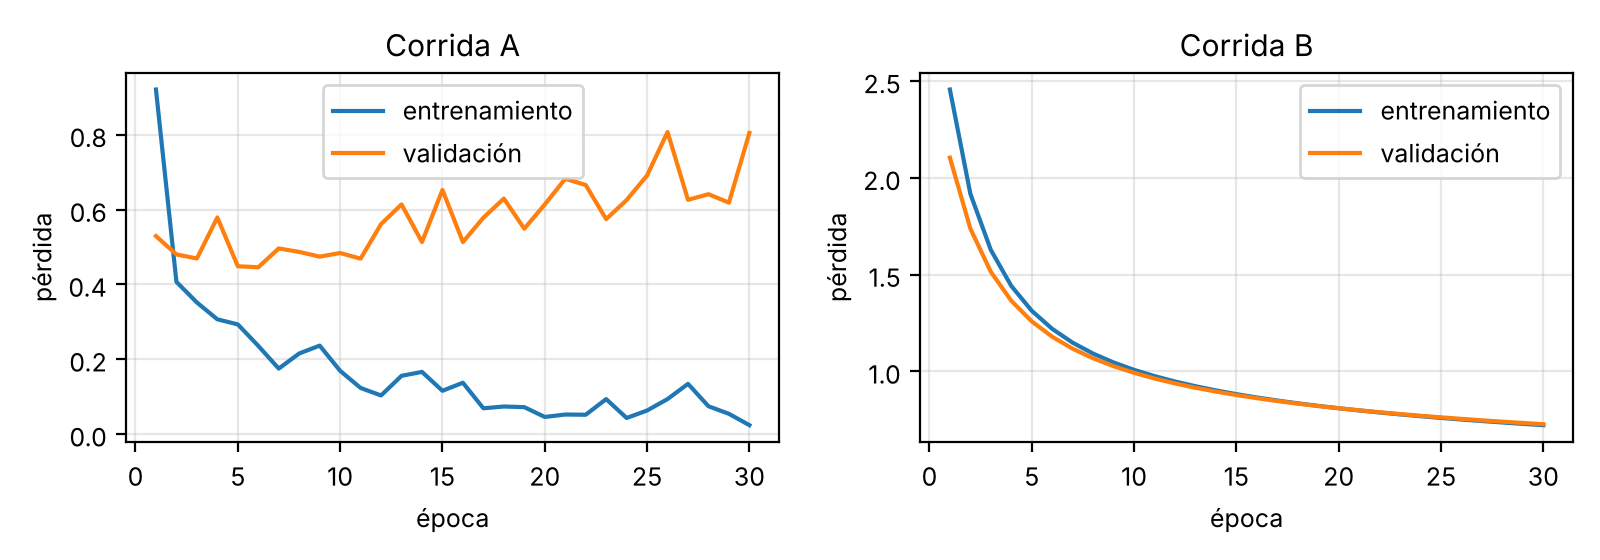
\includegraphics[width=\linewidth]{fig1_curvas.png}
\begin{enumerate}
\item Diagnostica cada corrida en una frase, citando lo que ves en las curvas.\resp{3.2cm}
\item Propón \textbf{una} acción para cada corrida y di qué cambio en las curvas confirmaría que funcionó.\resp{3.2cm}
\end{enumerate}

\preg{2. Un cálculo de varianza}
Una capa ReLU con $n_\mathrm{in}=400$ y pesos $W\sim\mathcal N(0,\,0.05^2)$. Supón que ReLU conserva la mitad de la varianza.
\begin{enumerate}
\item ¿Por qué factor se multiplica $\operatorname{Var}(a_l)$ en cada capa?\resp{1.8cm}
\item Después de 10 capas, ¿cuánto vale $\operatorname{std}(a_{10})$ en proporción a la inicial?\resp{1.8cm}
\item ¿Qué desviación estándar $\sigma$ conserva la varianza? ¿Cómo se llama esa inicialización?\resp{1.8cm}
\end{enumerate}

\newpage
\preg{3. Tres inicializaciones}
Un MLP de 15 capas ocultas con ReLU y 256 unidades, medido \textbf{antes de entrenar} sobre un lote, con tres inicializaciones: la de PyTorch por defecto, Xavier y He (en algún orden).\par
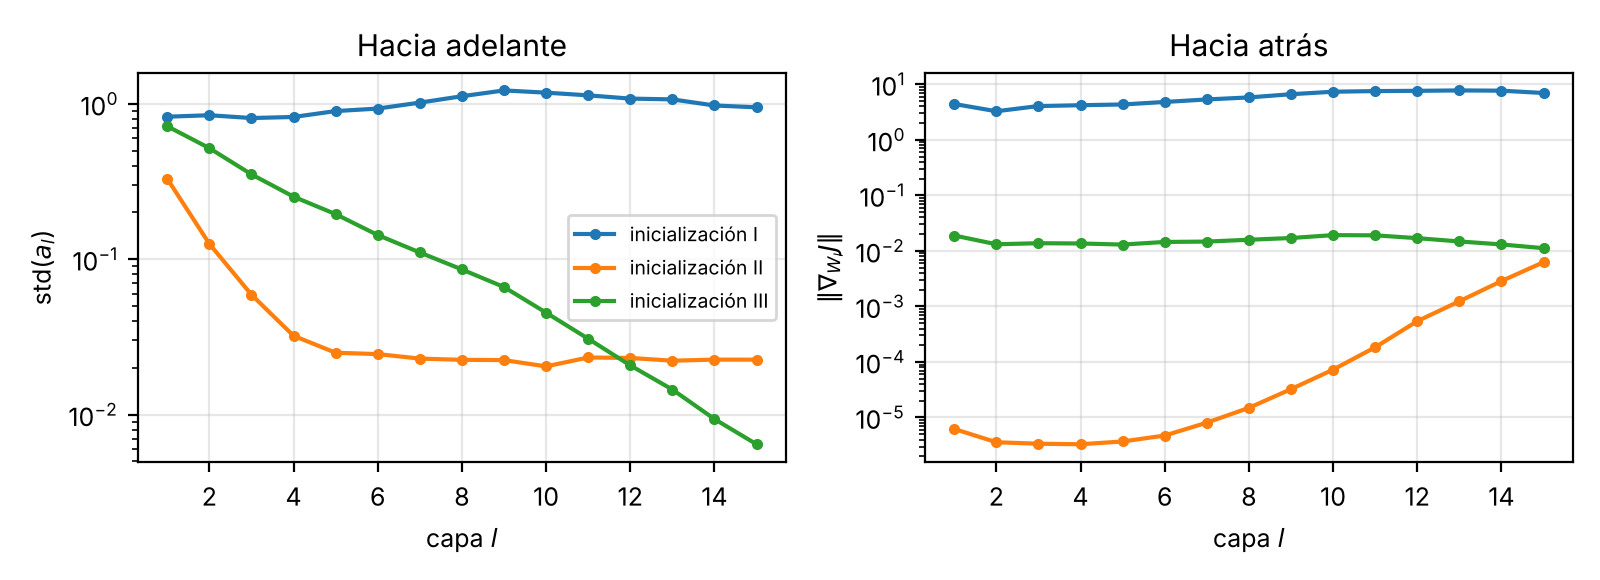
\includegraphics[width=\linewidth]{fig2_capas.png}
\begin{enumerate}
\item Asigna I, II y III a \{PyTorch por defecto, Xavier, He\}. Justifica cada una con un número de las gráficas.\resp{3.4cm}
\item ¿Cuál entrenarías con SGD? ¿Qué les pasaría a las primeras capas con las otras dos?\resp{2.4cm}
\end{enumerate}

\preg{4. La pérdida inicial}
Un problema con $C=7$ clases balanceadas. Tres compañeros reportan la pérdida de \textbf{validación antes de entrenar} (entropía cruzada). Interpreta cada valor en una frase: ¿está bien? Si no, ¿qué sospechas?
\begin{enumerate}
\item 1.95\resp{1.4cm}
\item 38.2\resp{1.8cm}
\item 0.03\resp{1.8cm}
\end{enumerate}

\newpage
\preg{5. Tamaño del lote}
El mismo modelo con el mismo $\eta=0.05$ durante 3 épocas. Una corrida usa lotes de 16 y la otra lotes de 1024. Corrida P: 0.14 s por época. Corrida Q: 0.82 s por época.\par
\begin{center}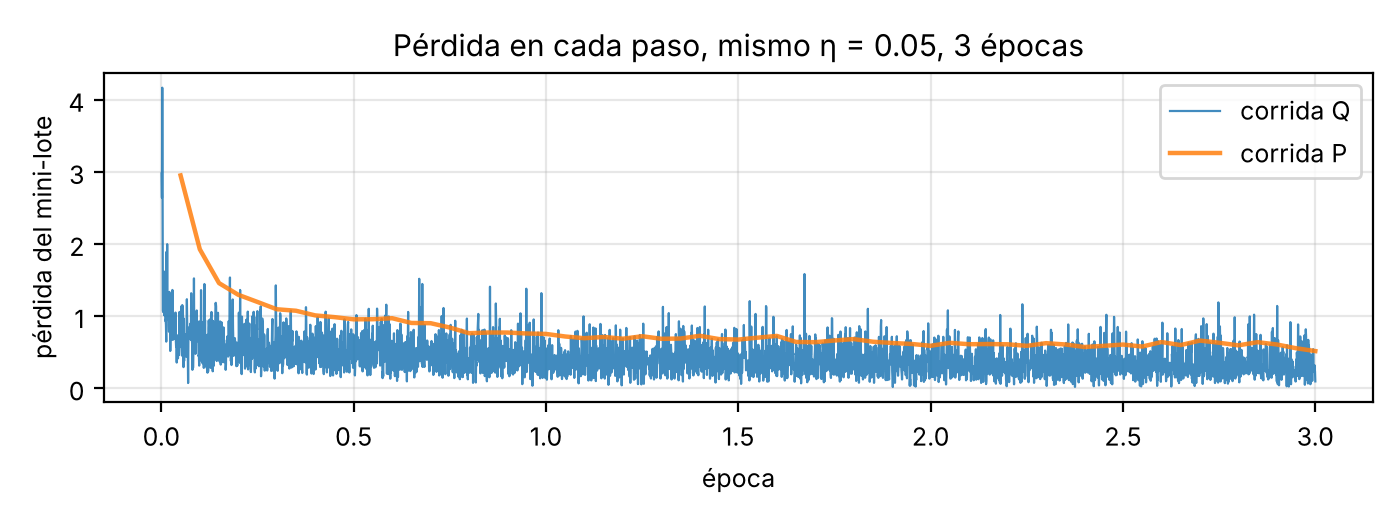
\includegraphics[width=0.85\linewidth]{fig3_lote.png}\end{center}
\begin{enumerate}
\item ¿Cuál corrida usa lotes de 16? Da dos razones que se vean en la figura o en los tiempos.\resp{5.5cm}
\item Si pasas de lotes de 16 a 1024 y quieres avanzar lo mismo por época, ¿qué haces con $\eta$? ¿Para qué sirve un \emph{warmup}?\resp{5.5cm}
\end{enumerate}

\newpage
\preg{6. Profundidad y weight decay}
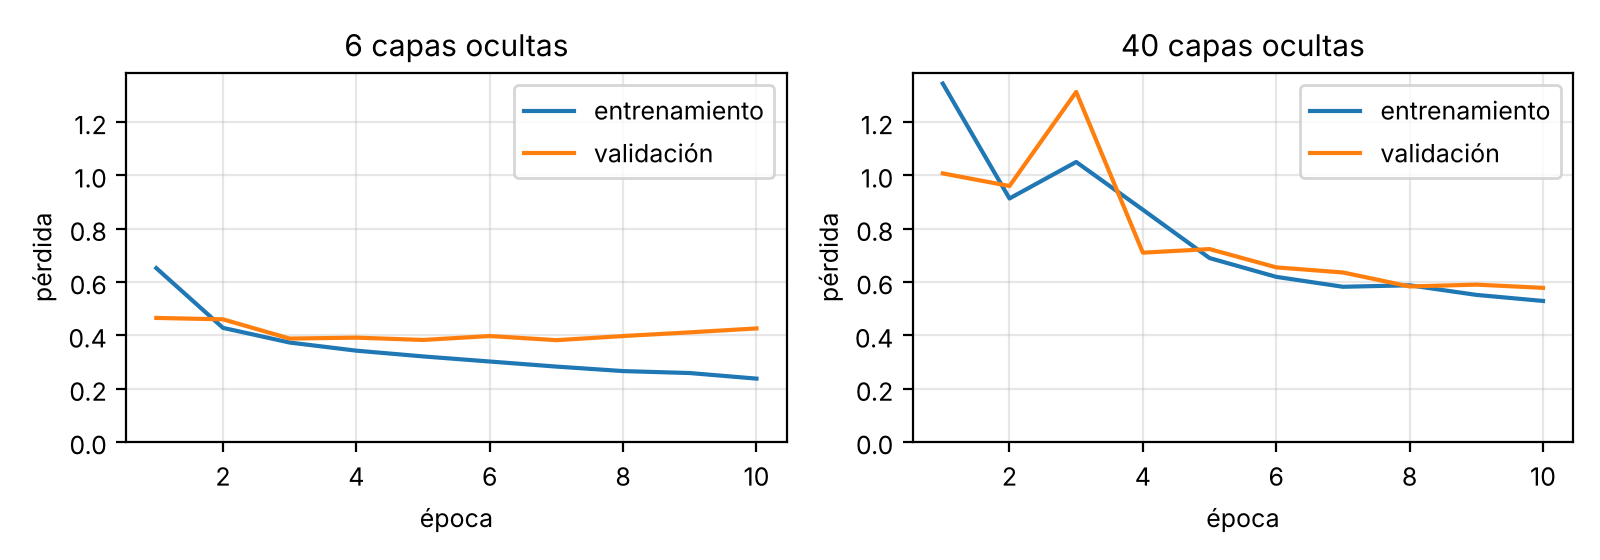
\includegraphics[width=\linewidth]{fig4_profundidad.png}
\begin{enumerate}
\item Un estudiante dice: «la red de 40 capas sobreajusta; hay que agregarle Dropout». ¿Estás de acuerdo? Justifica con las curvas y propón qué cambiarías.\resp{6cm}
\item \texttt{torch.optim.Adam(..., weight\_decay=λ)} frente a \texttt{torch.optim.AdamW(..., weight\_decay=λ)}: ¿qué hace cada uno con la penalización, y por qué se prefiere AdamW?\resp{4cm}
\end{enumerate}

\end{document}
